\documentclass[a4paper,fleqn]{cas-sc}

%Packages
\usepackage[authoryear,longnamesfirst]{natbib}
\usepackage[spanish]{babel}


%%%Author macros
\def\tsc#1{\csdef{#1}{\textsc{\lowercase{#1}}\xspace}}
\tsc{WGM}
\tsc{QE}
%%%

\newtheorem{theorem}{Theorem}
\newtheorem{lemma}[theorem]{Lemma}
\newdefinition{rmk}{Remark}
\newproof{pf}{Proof}
\newproof{pot}{Proof of Theorem \ref{thm}}


\begin{document}
\let\WriteBookmarks\relax
\def\floatpagepagefraction{1}
\def\textpagefraction{.001}

% Short title
\shorttitle{}    

% Short author
\shortauthors{Christian Paredes}  

% Main title of the paper
\title[mode = title]{Prociclicidad del Apalancamiento en el Sistema Financiero: Un Análisis de Datos de Panel Durante Períodos de Crisis}  

% Title footnote mark
\tnotemark[1]

% Title footnote 1.
\tnotetext[1]{Trabajo de econometría avanzada}

% First author

\author[1]{Christian L. Paredes Aguilera}%[
	%type=editor,
	%style=Español,
	%auid=001,
	%bioid=1,
	%prefix=Sir,
	%twitter=www.twitter.com/juanfidelalvarez,
	%linkedin=www.linkedin.com/in/juanfidelalvarez,
	%gplus=001]
%]

% Corresponding author indication
%\cormark[1]

% Footnote of the first author
%\fnmark[]

% Email id of the first author
% \ead{soyfode@gmail.com}

% URL of the first author
% \ead[url]{www.christianparedes.com}

% Credit authorship
%\credit{Conceptualization of this study, Methodology, Software}

% Address/affiliation
\affiliation[2]{organization={Universidad de Vigo},
            addressline={R\'ua as Pedreiras, 2}, 
            city={Vigo},
%           citysep={}, % Uncomment if no comma needed between city and postcode
            postcode={36310}, 
            %state={},
            country={España}}

%\credit{Data curation, Writing - Original draft preparation}

% For a title note without a number/mark
%\nonumnote{}

% Here goes the abstract
\begin{abstract}
    Este estudio explora la prociclicidad del apalancamiento en el sistema financiero, con un enfoque particular en los períodos de crisis. A través de un análisis detallado de los datos financieros, hemos observado que durante los períodos de crecimiento económico, las instituciones financieras tienden a aumentar su apalancamiento, lo que se revierte durante los shocks exógenos, resultando en una disminución de la oferta de crédito. Este comportamiento procíclico se mantiene constante a través de diferentes tipos de entidades financieras y durante períodos de dificultades financieras. Nuestro análisis proporciona una visión profunda de la dinámica del apalancamiento en el sistema financiero, destacando la influencia de factores externos, el entorno regulatorio, las estrategias empresariales y las condiciones del mercado.
\end{abstract}

% Use if graphical abstract is present
%\begin{graphicalabstract}
%\includegraphics{}
%\end{graphicalabstract}

% Research highlights
%\begin{highlights}
%\item 
%\item 
%\item 
%\end{highlights}

% Keywords
% Each keyword is seperated by \sep
\begin{keywords}
    Prociclicidad \sep Apalancamiento \sep Sistema Financiero \sep Análisis de Datos de Panel \sep Crisis de COVID-19 \sep Bancos Comerciales \sep Servicios Financieros 
\end{keywords}

\maketitle


% Main text
\section{Introducción}
En el contexto de la reciente pandemia de COVID-19 y las crisis financieras globales de 2007-2008, los sistemas financieros han experimentado cambios significativos. Estos eventos han puesto de manifiesto la importancia de entender la dinámica de los sistemas financieros y su interacción con la economía en general. Según el Banco de Pagos Internacionales (2008), la prociclicidad se refiere a las interacciones dinámicas entre el sistema financiero y los sectores reales de la economía. En contraposición a esto, los modelos tradicionales del acelerador financiero sostienen que la prociclicidad de los precios de los activos es la que explica las fases de expansión y recesión del ciclo económico (Bernanke y Gertler, 1989; Kiyotaki y Moore, 1997).

Nuestro estudio se propone analizar cómo las instituciones financieras gestionan sus balances en este contexto cambiante. Buscamos comprender el delicado equilibrio entre el crecimiento del apalancamiento y diversas variables económicas, como el crecimiento del tamaño y el crecimiento del valor de mercado. Este análisis se realiza para tres tipos diferentes de entidades financieras: bancos comerciales, servicios financieros y servicios financieros inmobiliarios.

El objetivo de nuestro trabajo es investigar el sistema financiero estadounidense en tres partes distintas. El primer paso consiste en la extracción de datos, con especial atención a la obtención de datos relevantes relacionados con varios componentes del sistema financiero. A continuación, procedemos a crear un conjunto de datos de panel adecuado, fusionando y estructurando los diferentes conjuntos de datos para garantizar su consistencia y coherencia. Luego, realizamos transformaciones logarítmicas, seguidas de una inspección detallada de las variables y el cálculo de estadísticas de resumen. La segunda parte de nuestro estudio se centra en la sensibilidad del coeficiente de apalancamiento al crecimiento del tamaño. Los coeficientes derivados de estas regresiones sirven como indicadores de su impacto y se interpretan en consecuencia. Además, también examinamos los indicadores de bondad de ajuste de cada regresión. El último segmento de nuestro análisis explora la prociclicidad del apalancamiento entre subperíodos y entidades financieras. Para ello, se realizan regresiones de panel para cada entidad y subperiodo. Al examinar las variaciones, tendencias e implicaciones observadas en estas regresiones, hemos obtenido valiosos datos sobre la dinámica del sistema financiero estadounidense.

Este estudio proporciona una visión integral de la gestión de los balances de las instituciones financieras y su interacción con la economía en general. Los resultados obtenidos podrían ser de gran utilidad para los responsables de la formulación de políticas, los reguladores financieros y los investigadores interesados en la dinámica de los sistemas financieros.

\section{Limpieza de datos y análisis descriptivo}

Nuestro estudio abarcó el periodo desde el cuarto trimestre de 2005 hasta el segundo trimestre de 2023, utilizando datos trimestrales de los sistemas financieros de Estados Unidos. El conjunto de datos que utilizamos incluía parámetros financieros para cada periodo de referencia y entidad, como los activos totales, el valor de mercado de las acciones, el precio, el ratio de apalancamiento y el ratio entre el valor de mercado y el valor contable. Sin embargo, nos encontramos con la ausencia de algunos valores en nuestro conjunto de datos, lo cual fue necesario abordar para nuestro análisis.

Para tratar los valores faltantes, recurrimos a técnicas de interpolación, utilizando los valores anteriores y posteriores al dato faltante para calcular un promedio que sirviera como sustituto del valor ausente. Posteriormente, añadimos las variables necesarias para nuestro análisis, como el logaritmo natural del apalancamiento y el crecimiento de los activos totales.

\begin{figure}[h]
    \centering
    \caption{Distribución por entidad}
    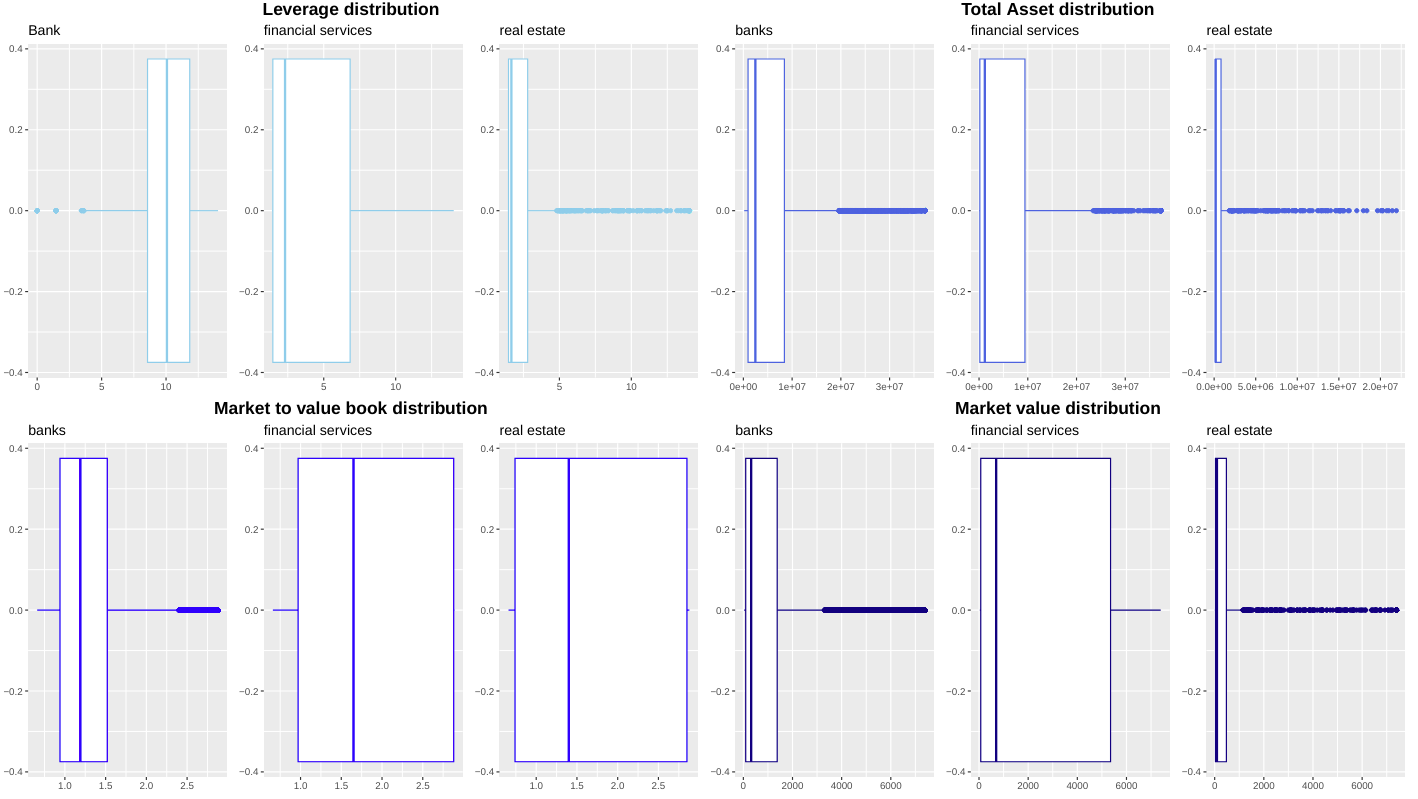
\includegraphics[width=1\textwidth]{gr1.png}
\end{figure}

\begin{table}[h]
    \centering
    \caption{Estadística descriptiva del conjunto de datos}
    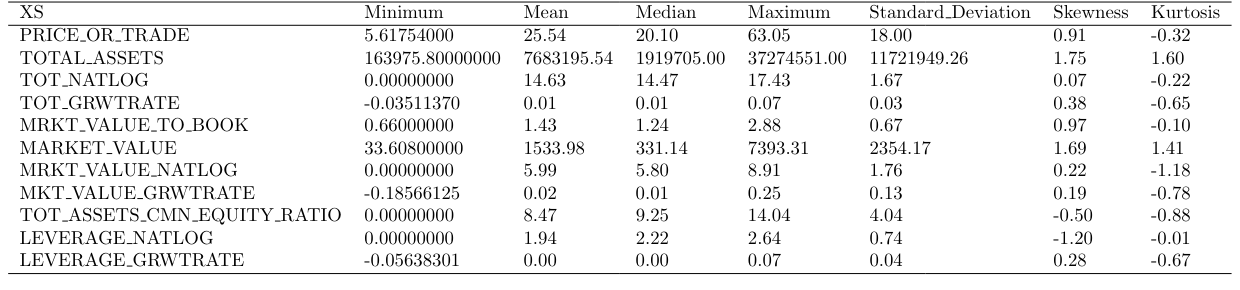
\includegraphics[width=1\textwidth]{tabla1.png}
\end{table}

Al centrarnos en un análisis comparativo entre bancos, servicios financieros y servicios financieros inmobiliarios, observamos que los servicios financieros en EE.UU. mostraron una media más alta en varias variables. Esto sugiere que los servicios financieros podrían ser generalmente mayores en términos de activos y capitalización de mercado en comparación con los bancos y los servicios financieros inmobiliarios. Además, estos valores más altos podrían indicar que los servicios financieros no sólo se perciben como más valiosos o se negocian más activamente, sino también como una mejor oportunidad de inversión debido a la mayor expansión del negocio. Sin embargo, es fundamental tener en cuenta que los servicios financieros también presentan una mayor variabilidad, lo que podría indicar un mayor riesgo en comparación con los bancos y los servicios inmobiliarios.

\begin{table}[h]
    \centering
    \caption{Estadística descriptiva para bancos}
    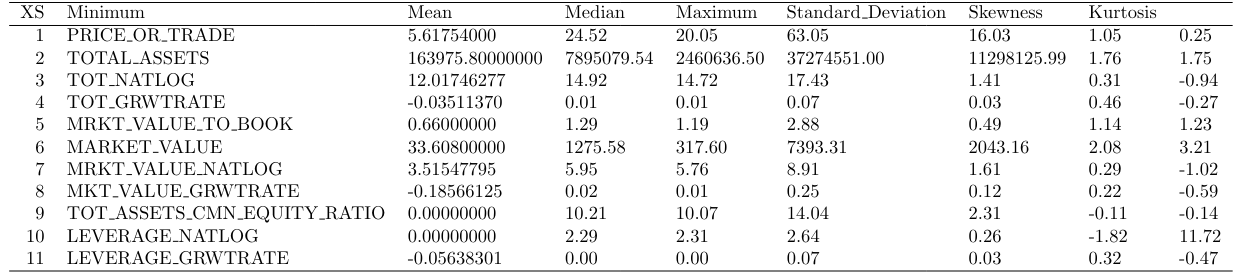
\includegraphics[width=1\textwidth]{tabla2.png}
\end{table}

A pesar de que los servicios financieros tienen medias más altas en otras variables, los bancos muestran la media más alta para el coeficiente de apalancamiento. Este resultado podría reflejar la naturaleza única de las operaciones bancarias, ya que los bancos podrían utilizar el apalancamiento como estrategia deliberada para amplificar los beneficios. De hecho, es importante recordar que los bancos suelen operar con estructuras de capital diferentes a las de otras entidades financieras. Pueden depender más de la financiación mediante deuda o tener razones reguladoras específicas para mantener un apalancamiento más elevado, debido a la naturaleza de sus operaciones, en las que el apalancamiento es una parte crucial de sus actividades de préstamo e inversión.

\begin{table}[h]
    \centering
    \caption{Estadística descriptiva para servicios financieros}
    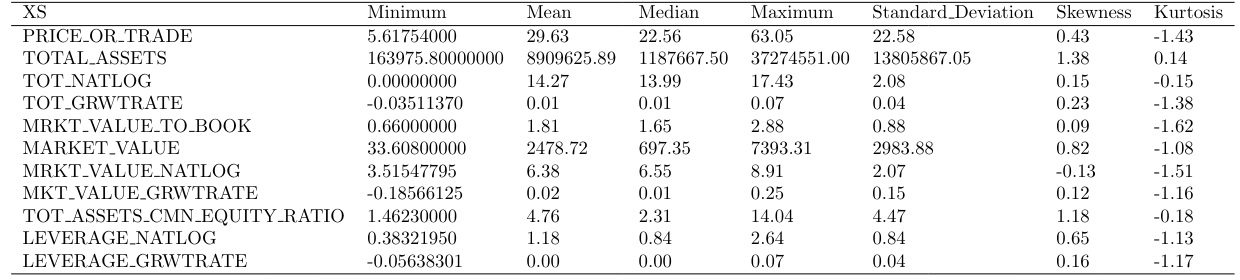
\includegraphics[width=1\textwidth]{tabla3.png}
\end{table}

Al estudiar la desviación estándar desde una perspectiva financiera, observamos que los servicios financieros presentaban desviaciones estándar más elevadas en la mayoría de las variables, lo que sugiere una mayor variabilidad y volatilidad dentro de este sector. Podrían experimentar fluctuaciones más significativas en los precios, los valores de mercado y las tasas de crecimiento en comparación con los bancos y los servicios inmobiliarios. Además, la desviación estándar más alta en los activos totales de los servicios financieros podría indicar una mezcla de instituciones financieras dentro del sector, incluyendo tanto grandes corporaciones como entidades más pequeñas con distintos modelos de negocio, enfoques de inversión o composición de activos.

Por último, observamos que los servicios inmobiliarios mostraron una desviación estándar más baja en comparación con los bancos y los servicios financieros, lo que podría indicar una menor variabilidad en sus operaciones y una mayor estabilidad en sus actividades financieras. Sin embargo, es importante tener en cuenta que esta menor variabilidad podría estar asociada a un menor crecimiento y a una menor capacidad para adaptarse a los cambios en el entorno económico y financiero.

\begin{table}[h]
    \centering
    \caption{Estadística descriptiva para servicios financieros inmobiliarios}
    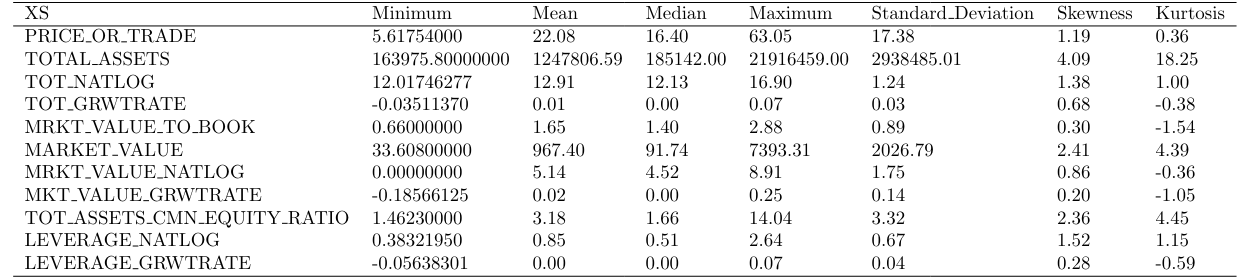
\includegraphics[width=1\textwidth]{tabla4.png}
\end{table}

En resumen, nuestro análisis descriptivo proporciona una visión detallada de la estructura y las características de los diferentes sectores del sistema financiero estadounidense. Estos hallazgos son fundamentales para entender la dinámica de estos sectores y proporcionan una base sólida para nuestro análisis posterior de la prociclicidad del apalancamiento y su impacto en el sistema financiero en general.

\section{Análisis de Panel a Largo Plazo}
En la segunda parte de nuestro estudio, nos enfocamos en analizar la sensibilidad del ratio de apalancamiento al crecimiento del tamaño. Para esta sección, utilizamos un conjunto de datos de panel completo que incluye tres entidades: bancos comerciales, servicios de financiación inmobiliaria y servicios financieros.
\subsection{Descripción del Modelo}
Para nuestro análisis, aplicamos cuatro modelos de regresión diferentes, todos ellos con el crecimiento del apalancamiento en el tiempo t como variable dependiente. En cada modelo, incluimos variables ficticias para cada año. Los modelos son los siguientes:

\begin{enumerate}[(1)]
    \item $\Delta \text{Apalancam}_{i,t} = \beta_0 + \beta_1 \Delta \text{TotalActivos}_{i,t} + \beta_2 \ln(\text{Apalancam}_{i,t-1}) + \sum\limits_{2023}^{2005} \text{año}$.

    \item $\Delta \text{Apalancam}_{i,t} = \beta_0 + \beta_1 \Delta \text{TotalActivos}_{i,t} + \beta_2 \text{MercadoALibros}_{i,t-1} + \beta_2 \ln(\text{Apalancam}_{i,t-1}) + \sum\limits_{2023}^{2005} \text{año}$.

    \item $Delta \text{Apalancam}_{i,t} = \beta_0 + \beta_1 \Delta \text{ValorDeMercado}_{i,t} + \beta_2 \ln(\text{Apalancam}_{i,t-1}) + \sum\limits_{2023}^{2005} \text{año}$.

    \item $\Delta \text{Apalancam}_{i,t} = \beta_0 + \beta_1 \Delta \text{ValorDeMercado}_{i,t} + \beta_2 \text{MercadoALibros}_{i,t-1} + \beta_2 \ln(\text{Apalancam}_{i,t-1}) + \sum\limits_{2023}^{2005} \text{año}$.

\end{enumerate}

En la primera regresión (1), las variables independientes son el crecimiento del tamaño en $t$ y el logaritmo natural del apalancamiento en el momento $t-1$. En la segunda regresión (2), las variables independientes son el crecimiento del tamaño en $t$, el valor de la relación entre el mercado y los libros en $t-1$ y el logaritmo natural del apalancamiento en $t-1$. En la tercera regresión (3), las variables independientes son la tasa de crecimiento del valor de mercado en $t$ y el logaritmo natural del apalancamiento en $t-1$. En la última regresión (4), las variables independientes son la tasa de crecimiento del valor de mercado en $t$, la relación entre el valor de mercado y el valor contable en $t-1$, y el logaritmo natural del apalancamiento en $t-1$.
Inicialmente, las estimaciones obtenidas de estas regresiones eran de baja calidad, y los principales indicadores estadísticos, como el coeficiente de determinación $R^2$ y el $R^2$ ajustado, eran muy bajos, cuando no negativos. Esto se debía a la presencia de numerosos valores atípicos en el conjunto de datos. Por lo tanto, procedimos a aplicar una técnica de winsorización, estableciendo un umbral inferior de $0.1$ y un umbral superior de $0.90$. Como resultado, la calidad de las estimaciones mejoró notablemente, y los indicadores estadísticos aumentaron. Este proceso de limpieza de datos fue esencial para obtener resultados más precisos y significativos en nuestro análisis.


\subsection{Análisis de los resultados}
\begin{table}[h]
	\centering
	\caption{Análisis de panel de periodo largo de tiempo.}
	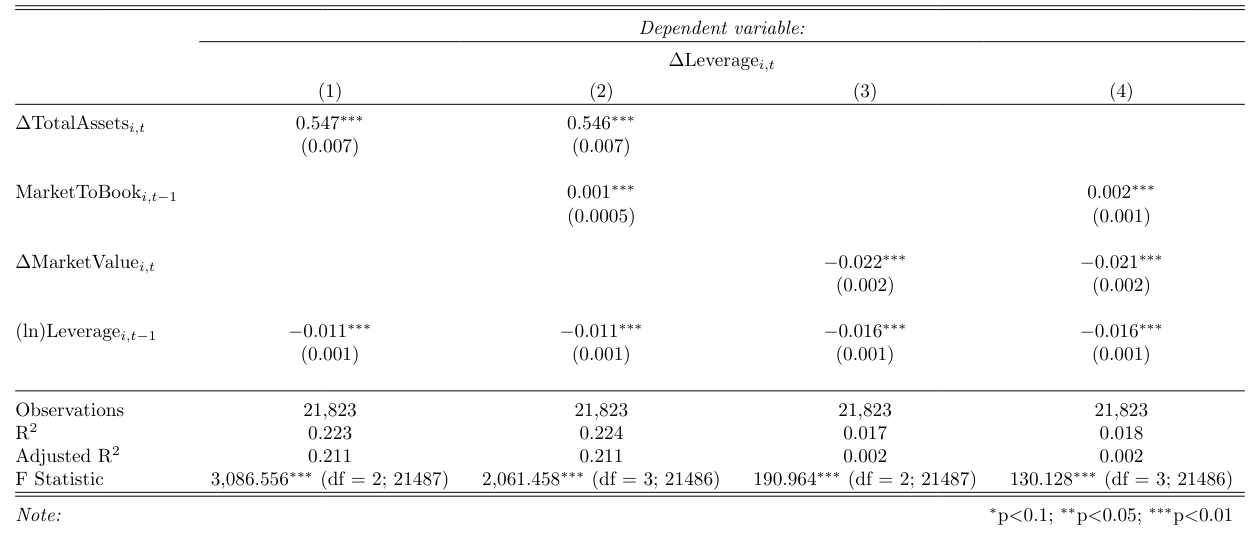
\includegraphics[width=1\textwidth]{tabla5.png}
\end{table}

Como se muestra en la Tabla 5, en las dos primeras regresiones - (1) y (2) - todos los regresores son estadísticamente significativos, con valores $t$ grandes y valores p muy pequeños. En ambos casos, se observa una relación fuerte y positiva entre las variables dependientes y las independientes. Esto constituye una prueba estadística sólida de su impacto en la tasa de crecimiento del apalancamiento. En cuanto a los indicadores de la bondad del ajuste, en ambos casos el $R^2$ es superior a $0.22$, y el $R^2$ ajustado es superior a $0.21$. Además, el valor p muy bajo ($<2.22e-16$) asociado al estadístico F de ambos modelos indica que los modelos son estadísticamente significativos.
En las dos últimas regresiones, (3) y (4), sustituimos la tasa de crecimiento por la tasa de crecimiento del valor de mercado. La relación entre la tasa de crecimiento del apalancamiento y todos los regresores - tasa de crecimiento del valor de mercado, ratio mercado/valor contable retardada, logaritmo natural retardado del apalancamiento - son altamente significativos desde el punto de vista estadístico. En cuanto al ajuste del modelo: el $R^2$ es superior a $0.017$ y el $R^2$ ajustado es de $0.002$, por lo que el modelo explica muy poco de la varianza de la variable dependiente. Sin embargo, el estadístico F es altamente significativo, lo que sugiere que los modelos son estadísticamente significativos.
En resumen, los resultados de la regresión indican que las variables independientes, entre ellas la tasa de crecimiento del valor de mercado, el logaritmo retardado del apalancamiento y las variables ficticias temporales, son estadísticamente significativas para explicar las variaciones de la tasa de crecimiento del apalancamiento. El hecho de que la tasa de crecimiento presente un coeficiente elevado y estadísticamente significativo lleva a la conclusión de que el crecimiento va acompañado de un aumento de los ingresos y los beneficios, por lo que el coeficiente de apalancamiento puede mejorar porque se amplía la base de fondos propios.
Desde un punto de vista financiero, una relación positiva entre el crecimiento del apalancamiento y el crecimiento del tamaño puede indicar que a las instituciones financieras más grandes les puede resultar ventajoso utilizar el apalancamiento para financiar sus operaciones y su expansión. A medida que un banco crece, por ejemplo, puede endeudarse más para financiar inversiones adicionales, conceder más préstamos o participar en otras actividades financieras. Sin embargo, la relación entre el crecimiento del apalancamiento y el crecimiento del tamaño en los bancos comerciales y las industrias de servicios financieros puede variar en función de diversos factores. Por ejemplo:

\begin{itemize}
    \item \textbf{Estructura de capital:} La relación entre el crecimiento del tamaño y el crecimiento del apalancamiento puede verse influida por el concepto de estructura óptima del capital. Las instituciones financieras suelen tratar de alcanzar un equilibrio entre deuda y capital para optimizar su coste de capital y minimizar el riesgo financiero. La estructura óptima de capital puede cambiar a medida que crece la institución y evolucionan factores externos como los tipos de interés y las condiciones económicas.
    \item \textbf{Entorno normativo:} El entorno normativo desempeña un papel importante en la configuración de la estructura de capital de los bancos y las instituciones financieras. Los requisitos normativos pueden influir en la cantidad de capital que los bancos deben mantener, afectando a sus decisiones en materia de apalancamiento. Los cambios normativos pueden influir en la relación observada entre el crecimiento del tamaño y el crecimiento del apalancamiento.
    \item \textbf{Estrategias empresariales:} Los distintos bancos pueden seguir estrategias de negocio diferentes, lo que puede influir en sus decisiones sobre la estructura de capital. Algunos bancos pueden utilizar activamente el apalancamiento para aumentar la rentabilidad y buscar oportunidades de crecimiento, mientras que otros pueden dar prioridad a un enfoque más conservador, centrándose en la estabilidad y la gestión del riesgo.
    \item Condiciones del mercado: Las condiciones del mercado, incluidos los tipos de interés, la estabilidad económica y la disponibilidad de crédito, pueden influir en la decisión de un banco sobre el apalancamiento. En periodos de expansión económica y condiciones de mercado favorables, los bancos pueden ser más proclives a apalancarse para crecer.
    \item \textbf{Condiciones del mercado:} Las condiciones del mercado, incluidos los tipos de interés, la estabilidad económica y la disponibilidad de crédito, pueden influir en la decisión de un banco sobre el apalancamiento. En periodos de expansión económica y condiciones de mercado favorables, los bancos pueden ser más proclives a apalancarse para crecer.
\end{itemize}


\section{Análisis de Panel por Entidad y Periodos de Dificultad}

En la última parte de nuestra investigación, examinamos la prociclicidad del apalancamiento para cada entidad financiera y determinamos si está presente durante los periodos de dificultades financieras en el mercado financiero.

\subsection{Descripción del Modelo}

Primero, definimos un modelo con un tipo de entidad financiera como variable ficticia para analizar el posible efecto que podrían tener diferentes modelos de negocio de entidades financieras sobre el crecimiento del apalancamiento:

\begin{enumerate}[(5)]
    \item $\Delta \text{Apalancam}_{i,t} = \beta_0 + \beta_1 \Delta \text{ActivosTotales}_{i,t} + \beta_2 \ln(\text{apalancam}_{i,t-1}) + \beta_3 \text{MercadoALibros}_{i,t-1} + \beta_4 \text{ServicioFinanciero}_{i,t} + \beta_5 \text{ServicioFinancieroDeBienesRaíces}_{i,t} + \sum\limits_{2005}^{2023} \text{año}$
\end{enumerate}

Donde Servicios Financieros $i,t$ toma el valor 1 en el trimestre $t$ cuando la entidad financiera $i$ es una entidad de servicios financieros y $0$ en caso contrario y Bienes Raíces FS $i,t$ cuando la entidad financiera $i$ es una entidad de financiación inmobiliaria y 0 en caso contrario. Además, este modelo controla el tiempo ficticio.
En segundo lugar, para capturar el comportamiento diferente sobre la prociclicidad de cada tipo de entidad financiera, creamos efectos marginales:

\begin{enumerate}[(6)]
    \item $\Delta \text{Apalancam}_{i,t} = \beta_0 + \beta_1 \Delta \text{ActivosTotales}_{i,t} + \beta_2 \ln(\text{apalancam}_{i,t-1}) + \beta_3 \text{MercadoALibros}_{i,t-1} + \beta_4 \text{CrecimienTamaño} \times \text{NoBancos}_{i,t}$
\end{enumerate}

Donde CrecimientoDelTamañoxNoBancos i,t representa un efecto marginal en el que noBancos toma el valor 1 cuando la entidad financiera es una entidad de servicios financieros o una entidad de financiación inmobiliaria. Su coeficiente sugiere si la prociclicidad en el apalancamiento está más presente en los bancos que en las instituciones financieras que están relacionadas con otro tipo de actividad financiera. Para confirmar los resultados se consideran los siguientes efectos marginales:

\begin{enumerate}[(7)]
    \item $\Delta \text{Apalancam}_{i,t} = \beta_0 + \beta_1 \Delta \text{ActivosTotales}_{i,t} + \beta_2 \ln(\text{apalancam}_{i,t-1}) + \beta_3 \text{MercadoALibros}_{i,t-1} + \beta_4 \text{CrecimienTamaño} \times \text{ServiciosFinancieros}_{i,t} + \beta_5 \text{CrecimienTamaño} \times \text{BienesRaíces}_{i,t}$
\end{enumerate}

Donde CrecimienTamañoxServiciosFinancieros y CrecimienTamañoxBienesRaíces representan el efecto marginal para el cual la variable Finance Services toma el valor 1 cuando la entidad I es una entidad de servicios financieros, 0 en caso contrario y Real Estate toma el valor 1 cuando la entidad I es una entidad financiera de bienes raíces, 0 en caso contrario.
Para el estudio, si la prociclicidad del apalancamiento está presente en períodos de dificultades financieras, se eligió la crisis financiera de 2008 y la crisis de Covid-19 para estimar el siguiente modelo para cada período de crisis:

\begin{enumerate}[(8)]
    \item $\Delta \text{Apalancamiento}_{i,t} = \beta_0 + \beta_1 \Delta \text{Tamaño}_{i,t} + \beta_2 \ln(\text{apalancamiento}_{i,t-1}) + \beta_3 \text{MercadoALibros}_{i,t-1}$
\end{enumerate}

El período de crisis para el análisis de la crisis financiera de 2008 es de 2007 a 2009 y para el análisis de la crisis de Covid-19 de 2020 a 2022. Estos modelos nos permitirán entender cómo las diferentes entidades financieras y los periodos de dificultades financieras pueden afectar la prociclicidad del apalancamiento. Los resultados de estos análisis proporcionarán una visión más profunda de la dinámica del sistema financiero estadounidense durante los periodos de crisis.


\subsection{Resultados}
Los resultados obtenidos de la ecuación (5), presentados en la columna 1 del Cuadro 6, proporcionan una visión valiosa de la prociclicidad del apalancamiento en las instituciones financieras. El coeficiente estimado para el crecimiento del tamaño es positivo y altamente significativo, lo que indica una fuerte relación positiva entre el crecimiento del tamaño de una institución financiera y su nivel de apalancamiento. Este hallazgo respalda la teoría de la prociclicidad del apalancamiento, sugiriendo que las instituciones financieras tienden a aumentar su apalancamiento durante los periodos de crecimiento económico.

Además, el coeficiente de la Relación Valor de Mercado a Valor Contable es positivo, aunque pequeño, lo que indica que un aumento en el valor de mercado en relación con el valor en libros está asociado con un aumento en el crecimiento del apalancamiento. Este resultado puede reflejar la percepción de los inversores de que las instituciones financieras con un mayor valor de mercado son menos riesgosas, lo que les permite aumentar su apalancamiento.

Por otro lado, el logaritmo natural del apalancamiento del trimestre anterior presenta un coeficiente negativo, lo que sugiere que las instituciones financieras que tenían un alto nivel de apalancamiento en el pasado tienden a reducir su apalancamiento en el futuro. Este hallazgo puede reflejar la gestión del riesgo de las instituciones financieras, que buscan mantener su apalancamiento dentro de un rango aceptable para minimizar su exposición al riesgo.

En cuanto al análisis de los efectos de cada tipo de entidad financiera, los coeficientes negativos para los Servicios Financieros y los Servicios Financieros Inmobiliarios sugieren que los bancos tienden a tener un mayor crecimiento del apalancamiento que estas entidades. Este resultado puede reflejar las diferencias en los modelos de negocio y las estructuras de capital de estas entidades.

\begin{table}[h]
	\centering
	\caption{Análisis de datos de panel de resultados para la prociclicidad del apalancamiento por tipo de entidad}
	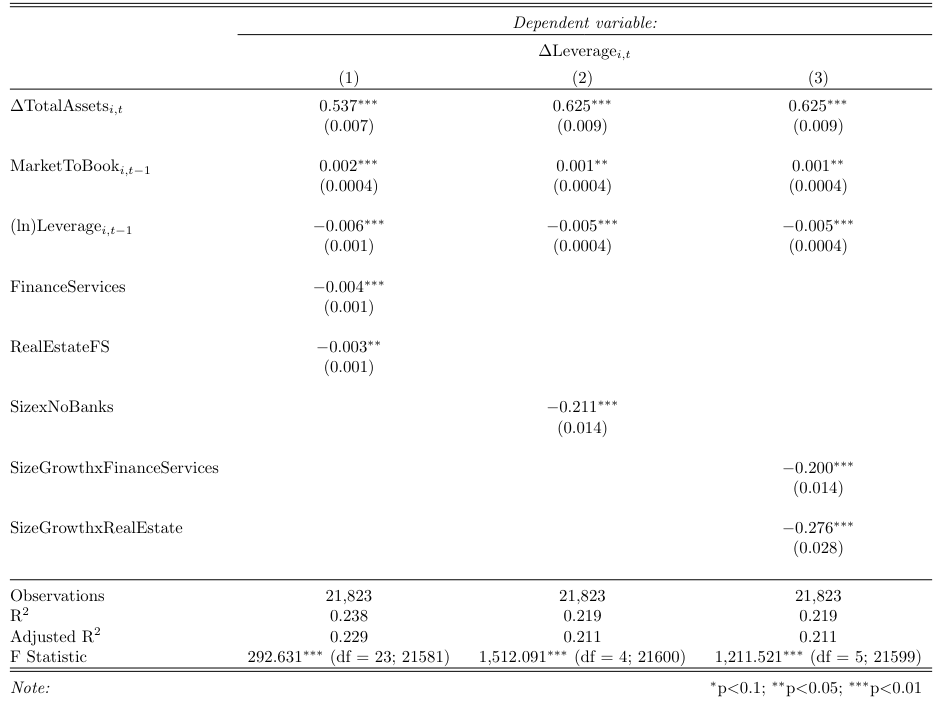
\includegraphics[width=.815\textwidth]{tabla6.png}
\end{table}

En las ecuaciones (6) y (7), introducimos efectos marginales para capturar diferentes comportamientos de prociclicidad entre los diferentes tipos de entidades financieras. Los resultados confirman que los bancos tienden a tener una mayor prociclicidad del apalancamiento que las entidades de servicios financieros y las entidades de servicios financieros inmobiliarios.

Finalmente, en la ecuación (8), examinamos si la prociclicidad del apalancamiento está presente durante los periodos de dificultades financieras, utilizando como casos de estudio la crisis financiera de 2008 y la crisis de Covid-19. Los resultados indican que la prociclicidad del apalancamiento se mantiene durante estos periodos, lo que sugiere que las instituciones financieras continúan aumentando su apalancamiento durante las crisis financieras.

\begin{table}[h]
	\centering
	\caption{Análisis de datos del panel de resultados para la prociclicidad del apalancamiento por períodos de dificultades financieras}
	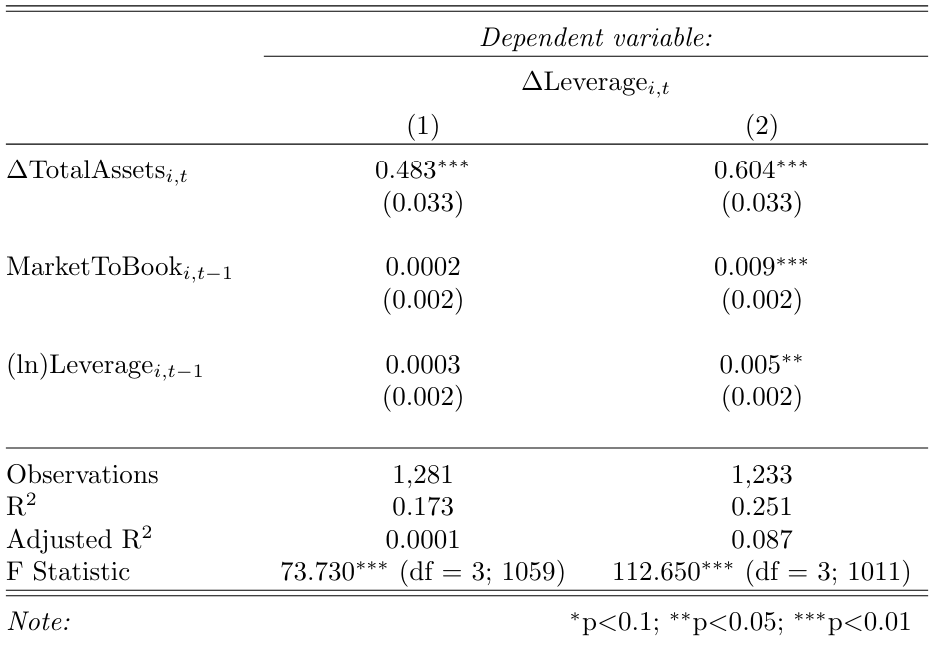
\includegraphics[width=.6\textwidth]{tabla7.png}
\end{table}

Estos hallazgos proporcionan una visión valiosa de la dinámica del apalancamiento en las instituciones financieras y pueden tener implicaciones importantes para la gestión del riesgo y la regulación financiera. Sin embargo, es importante tener en cuenta que estos resultados son preliminares y que se necesitan más investigaciones para confirmar estos hallazgos y explorar más a fondo las dinámicas del apalancamiento en las instituciones financieras.

En particular, sería útil investigar más a fondo la relación entre el crecimiento del tamaño y el apalancamiento en diferentes tipos de instituciones financieras. Además, sería interesante examinar cómo las políticas gubernamentales y las intervenciones durante las crisis financieras pueden afectar la prociclicidad del apalancamiento. Estas son áreas potenciales para futuras investigaciones.


\subsection{Conclusiones}
Nuestro análisis ha revelado una naturaleza procíclica inherente en el sistema financiero, caracterizada por un aumento del apalancamiento durante los períodos de crecimiento económico y una disminución durante los shocks exógenos. Este comportamiento se observa en diferentes tipos de entidades financieras, incluyendo bancos comerciales, servicios financieros y servicios de financiación inmobiliaria. Además, nuestros hallazgos indican que este comportamiento procíclico persiste incluso durante los períodos de dificultades financieras, como la crisis financiera de 2008 y la crisis de COVID-19. Estos resultados subrayan la importancia de considerar la prociclicidad del apalancamiento en la gestión del riesgo y la regulación financiera. Sin embargo, también destacan la necesidad de una mayor investigación para entender completamente las implicaciones de este comportamiento y desarrollar estrategias efectivas para mitigar sus posibles efectos negativos. En resumen, nuestro estudio proporciona una valiosa contribución a la comprensión de la dinámica del apalancamiento en el sistema financiero y sienta las bases para futuras investigaciones en este campo.


\section{Referencias}
\begin{itemize}
    \item Bernanke, B. S., y Gertler, M. (1989). Agency costs, net worth, and business fluctuations. American Economic Review, 79(1), 14-31.
    \item Kiyotaki, N., y Moore, J. (1997). Credit cycles. Journal of Political Economy, 105(2), 211-248.
\end{itemize}

% To print the credit authorship contribution details
%\printcredits

%\bibliographystyle{cas-model2-names}

% Loading bibliography database
%\bibliography{refs}

% Biography
%\bio{}
% Here goes the biography details.
%\endbio


\end{document}

